\documentclass[t, aspectratio=169]{beamer}
\usepackage{amsmath,amsfonts,amsthm,amstext,amssymb, xcolor, tikz, pgf, mathrsfs, polynom, pifont, tabto}

% ----------------------------------------------------------
% Theme Setup

% Use Metropolis Theme
\usetheme[numbering=fraction]{metropolis}
\setbeamertemplate{blocks}[rounded][shadow=false]
\makeatletter
\setlength{\metropolis@titleseparator@linewidth}{1pt}
\makeatother

% Define Colors
\definecolor{chargerblue}{HTML}{002764}
\definecolor{chargerred}{HTML}{e02034}
\definecolor{bggray}{HTML}{d0d3d4}

% Set Colors
\setbeamercolor{title}{fg=chargerblue}
\setbeamercolor{background canvas}{bg=white}
\setbeamercolor{title separator}{fg=chargerred}
\setbeamercolor{structure}{fg=chargerblue}
\setbeamercolor{frametitle}{fg=white, bg=chargerblue}
\setbeamercolor*{normal text}{fg=chargerblue}
\setbeamercolor*{block body}{bg=bggray}
\setbeamercolor*{block title}{bg=chargerblue, fg=white}
% ----------------------------------------------------------

% ----------------------------------------------------------
% Custom Definitions, Commands, Environments, etc.

% Sets of numbers
\def\R{\mathbb{R}} % The reals
\def\N{\mathbb{N}} % The naturals
\def\Z{\mathbb{Z}} % The integers
\def\Q{\mathbb{Q}} % The rationals

% Blank space
\newcommand{\blank}[1]{\underline{\hspace{#1}}} % Blank space

% Change font colors
\newcommand{\cyan}[1]{{\color{cyan}{#1}}} % Changes font to cyan
\newcommand{\red}[1]{{\color{red}{#1}}} % Changes font to red
\newcommand{\magenta}[1]{{\color{magenta}{#1}}} % Changes font to magenta
\newcommand{\orange}[1]{{\color{orange}{#1}}} % Changes font to orange
\newcommand{\yellow}[1]{{\color{yellow}{#1}}} % Changes font to yellow
\newcommand{\violet}[1]{{\color{violet}{#1}}} % Changes font to violet
\newcommand{\green}[1]{{\color{green}{#1}}} % Changes font to green
\newcommand{\blue}[1]{{\color{blue}{#1}}} % Changes font to blue
\newcommand{\white}[1]{{\color{white}{#1}}} % Changes font to white

% Fitted inclusion symbols
\newcommand{\fp}[1]{\left({#1}\right)} % Fitted parentheses around content
\newcommand{\fb}[1]{\left[{#1}\right]} % Fitted brackets
\newcommand{\lhoi}[1]{\left({#1}\right]} % Left half-open interval
\newcommand{\rhoi}[1]{\left[{#1}\right)} % Right half-open interval
\newcommand{\set}[1]{\left\{{#1}\right\}} % Fitted braces (useful for sets)
\newcommand{\av}[1]{\left|{#1}\right|} % Fitted absolute value bars

% Augmented Matrix Environment
\newenvironment{amatrix}[1]{%
	\left[\begin{array}{@{}*{#1}{c}|c@{}}
	}{%
	\end{array}\right]
}

% Miscellaneous
\def\then{\Rightarrow}
\def\to{\rightarrow}
\def\d{^{\circ}}
\newcommand{\?}{\stackrel{?}{=}}
\newcommand{\cmark}{\text{ \ding{51}}}
\newcommand{\xmark}{\text{ \ding{55}}}

% Coordinate Plane (Four-Quadrant)
\def\coordplane {
	\begin{tikzpicture}        \draw[step=0.25cm,black,very thin,opacity=0.25] (-2.5cm, -2.5cm) grid (2.5cm, 2.5cm);
		\draw[<->,thick,black] (-2.5cm, 0) -- (2.5cm, 0) node[anchor=north west,pos=0.94,font=\scriptsize]{$x$};
		\draw[<->,thick,black] (0,-2.5cm) -- (0, 2.5cm) node[anchor=south east,font=\scriptsize,pos=0.94]{$y$};
	\end{tikzpicture}
}

% Coordinate Plane (One-Quadrant)
\def\onequad {
	\begin{tikzpicture}
		\draw[step=0.25cm, black, very thin, opacity=0.25] (0,0) grid (7.5cm,5cm);
		\draw[->, thick, black] (0,0) -- (7.5cm, 0) node[anchor=north west,font=\scriptsize,pos=0.94]{$x$};
		\draw[->, black, thick] (0,0) -- (0,5cm) node[anchor=south east,font=\scriptsize,pos=0.94]{$y$};
	\end{tikzpicture}
}
% ----------------------------------------------------------

% ----------------------------------------------------------
% Presentation Information
\title[5-2b]{Variance, Standard Deviation, and Expectation}
\subtitle{Section 5-2}
\author{Jacob Ayers}
\institute{Lesson \#15}
\date{MAT 110}
% ----------------------------------------------------------

\begin{document}
	
	% Slide 1 (Title Slide)
	\begin{frame}
		\titlepage
	\end{frame}
	
	% Slide 2 (Objectives)
	\begin{frame}{Objectives}
		\begin{itemize}
			\item Find the variance and standard deviation of a probability distribution
			\item Find the expectation of a probability distribution
		\end{itemize}
	\end{frame}

	\begin{frame}{Variance and Standard Deviation}
		While the mean of a distribution is useful, it doesn't give us any information about the spread of the distribution.
		
		If we want to know how much variation there is in a distribution, we use the variance and standard deviation. \pause
		
		The formulas for the variance and standard deviation of a probability distribution are as follows: \\
		
		$\sigma^2 = \sum\fb{X^2 \cdot P(X)} - \mu^2$ \\
		$\sigma = \sqrt{\sigma^2} = \sqrt{\sum\fb{X^2 \cdot P(X)} - \mu^2}$
		
		As with the mean, a graphing calculator will take care of the computations for us.
	\end{frame}

	\begin{frame}{Variance and Standard Deviation}
		A fitness center bought a new exercise machine called the Mountain Climber. They decided to keep track of hwo many people used the machine over a 3-hour period. If $X$ is the number of people who used the machine, find the variance and standard deviation of the probability distribution.
		
		\begin{tabular}{c|ccccc}
			$X$ & 0 & 1 & 2 & 3 & 4 \\ \hline
			$P(X)$ & 0.1 & 0.2 & 0.4 & 0.2 & 0.1
		\end{tabular} \pause
	
		Using a graphing calculator: \pause \\
		$\sigma \approx 1.1$ \pause \\
		$\sigma^2 = 1.095445115^2 = 1.2$ \pause
	\end{frame}

	\begin{frame}{Variance and Standard Deviation}
		First, add an $X^2$ row to our table since that's needed in the formula.
		
		\begin{tabular}{c|ccccc}
			$X$ & 0 & 1 & 2 & 3 & 4 \\ \hline
			$X^2$ & 0 & 1 & 4 & 9 & 16 \\ \hline 
			$P(X)$ & 0.1 & 0.2 & 0.4 & 0.2 & 0.1
		\end{tabular} \pause
	
		We also need the mean for our formula, so we'll need to calculate that first.
		\begin{flalign*}
			\mu &= \sum (X \cdot P(X)) & \\
			&= 0(0.1) + 1(0.2) + 2(0.4) + 3(0.2) + 4(0.1) & \\
			&= 2.0
		\end{flalign*}
	\end{frame}

	\begin{frame}{Variance and Standard Deviation}
		\begin{tabular}{c|ccccc}
			$X$ & 0 & 1 & 2 & 3 & 4 \\ \hline
			$X^2$ & 0 & 1 & 4 & 9 & 16 \\ \hline 
			$P(X)$ & 0.1 & 0.2 & 0.4 & 0.2 & 0.1
		\end{tabular}
		
		\onslide<2->{The formula for the variance is $\sigma^2 = \sum\fb{X^2 \cdot P(X)} - \mu^2$. Since $\mu = 2$, $\mu^2 = 4$. \\}
		\onslide<3->{We'll find $\sum\fb{X^2 \cdot P(X)}$, then subtract 4.}
		\begin{flalign*}
			\onslide<4->{\sum\fb{X^2 \cdot P(X)} &= 0(0.1) + 1(0.2) + 4(0.4) + 9(0.2) + 16(0.1) & \\}
			\onslide<5->{&= 5.2}
		\end{flalign*}
		\onslide<6->{So $\sigma^2 = 5.2 - 4 = 1.2$. \\}
		\onslide<7->{$\sigma = \sqrt{1.2} \approx 1.1$}
	\end{frame}

	\begin{frame}{Variance and Standard Deviation}
		A pizza shop owner determines the number of pizzas that are delivered each day. Find the mean, variance, and standard deviation for the distribution.
		
		\begin{tabular}{c|ccccc}
			$X$ & 35 & 36 & 37 & 38 & 39 \\ \hline
			$P(X)$ & 0.1 & 0.2 & 0.3 & 0.3 & 0.1
		\end{tabular} \pause
	
		Using a graphing calculator: \\
		$\mu = 37.1$ \\
		$\sigma \approx 1.1$ \\
		$\sigma^2 = 1.135781669^2 \approx 1.3$
	\end{frame}

	\begin{frame}{Expectation}
		The \textit{expectation}, or \textit{expected value}, of a probability distribution is the theoretical average value of the variable. \pause
		
		``Expectation" and ``mean" are two ways of talking about the same thing. So we calculate them using the same formula. \pause
		
		$\mu = E(X) = \sum (X \cdot P(X))$
	\end{frame}

	\begin{frame}{Expectation}
		One thousand tickets are sold at \$1 each for a raffle in which the grand prize is a smart TV valued at \$750. Find the expected value of purchasing one ticket for the raffle. \pause
		
		First, we make a probability distribution for the situation.
		
		\begin{tabular}{c|cc}
			Gain $X$ & \$749 & -\$1 \\ \hline
			Probability $P(X)$ & 0.001 & 0.999
		\end{tabular} \pause
		
		Now, find the expectation either by hand or with a calculator: $E(X) = -\$0.25$
	\end{frame}

	\begin{frame}{Expectation}
		A roulette wheel has 38 numbers (1 through 36, 0, and 00). Half of the numbers from 1-36 are red, and the other half are black. 0 and 00 are green. A ball is rolled, and it falls into one of the 38 slots, giving a winning number and a color. The payoffs for a \$1 bet are as follows:
		
		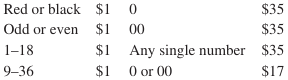
\includegraphics[width=3in]{roulette.png}
		
		If a person bets \$1, find the expected value for each.
		
		a) Red \tabto{0.5\textwidth} b) Even \\ c) Any single number \tabto{0.5\textwidth} d) 0 or 00
	\end{frame}

	\begin{frame}{Expectation}
		a) Red \pause
		
		If we bet on red, there are 18 ways ($36 \cdot \frac12$) we can win (+\$1), and 20 ways (38 - 18) we can lose (-\$1). So the probability distribution is as follows: \pause
		
		\begin{tabular}{c|cc}
			$X$ & 1 & -1 \\ \hline
			$P(X)$ & 18/38 & 20/38
		\end{tabular} \pause
	
		Using a calculator: $E(X) \approx -0.05$. You expect to lose about 5.26 cents. \pause
		
		b) Even \pause
		
		This is the exact same scenario as betting on red; there are 18 cases where you win a dollar, and 20 cases where you lose a dollar. No need to do the math again; you expect to lose about 5.26 cents.
	\end{frame}

	\begin{frame}{Expectation}
		c) Any single number \pause
		
		There is only one way we can win this bet (+\$35) and there are 37 ways to lose (-\$1). So the probability distribution is as follows: \pause
		
		\begin{tabular}{c|cc}
			$X$ & \$35 & -\$1 \\ \hline
			$P(X)$ & 1/38 & 37/38
		\end{tabular} \pause
	
		Using a calculator, $E(X) \approx -0.05$. You expect to lose about 5.26 cents. \pause
		
		d) 0 or 00
		
		There are two ways of winning (+\$17) and 36 ways of losing (-\$1). \pause
		
		\begin{tabular}{c|cc}
			$X$ & \$17 & -\$1 \\ \hline
			$P(X)$ & 2/38 & 36/38
		\end{tabular} \pause
	
		Using a calculator, $E(X) \approx -0.05$. You expect to lose about 5.26 cents.
	\end{frame}

	\begin{frame}{Expectation}
		A financial advisor suggests that his client select one of two types of bonds in which to invest \$5000. Bond $X$ pays a return of 4\%, and has a default rate of 2\%. Bond $Y$ has a 2.5\% return and a default rate of 1\%. Which investment is better? Note: if a bond defaults, the investor loses the entire investment. \pause
		
		This question can be answered using expected values.
		
		For bond $X$, the return is $5000 \cdot 0.04 = \$200$ if the bond doesn't default, and a loss of \$5000 if it does.
		
		\begin{tabular}{c|cc}
			$X$ & 200 & -5000 \\ \hline
			$P(X)$ & 0.98 & 0.02
		\end{tabular} \pause
	
		By hand: $E(X) = 200(.98) - 5000(0.02) = \$96$
	\end{frame}

	\begin{frame}{Expectation}
		For bond $Y$, the return is $5000 \cdot 0.025 = \$125$ if the bond doesn't default, and a loss of \$5000 if it does.
		
		\begin{tabular}{c|cc}
			$X$ & 125 & -5000 \\ \hline
			$P(X)$ & 0.99 & 0.01
		\end{tabular} \pause
	
		By hand: $E(X) = 125(0.99) - 5000(0.01) = \$73.75$ \pause
		
		The increased return rate more than outweighs the increased default risk; bond $X$ is the better investment.
	\end{frame}

	\begin{frame}{Next Steps}
		\begin{itemize}
			\item Complete Assignment \#7
			\item Begin Module \#9 \begin{itemize}
				\item Read 5-3
				\item Watch Video Lesson \#16
			\end{itemize}
		\end{itemize}
	
		\vfill
		
		Thanks for watching!
	\end{frame}
	
\end{document}